In this section, we will perform an analysis of certain important aspects and properties of our proposed algorithm with applications and limitations.

\subsection{Algorithm Applications}

Our proposed non-randomized algorithm can be extended beyond the field of solving this current problem. Some of the potential applications of our algorithm are:
\begin{itemize}
    \item \textbf{Recommendation Systems:} The algorithm has the ability to recommend different entities based on cost and reward modelling. Using this modelling property, this algorithm can be used for recommending different types of information after proper data representation.
    
    \item \textbf{Efficient Resource Allocation:} This algorithm can be used to perform a deeper analysis of space with supply-demand knowledge which can enhance the resource allocation process. Utilising cost constraint, rewards can be distributed efficiently resulting in a more effective resource allocation.
    
    \item \textbf{Ability to map any domain-related orienteering problem:} Our reward function can be enhanced to include any domain-related factors. This gives our algorithm the ability to work in any domain as the working only needs proper modelling of cost and reward functions. After proper modelling, our algorithm is mature enough to predict the required results with a great execution speed.
\end{itemize}

\subsection{Algorithm Data Requirements}

Our proposed algorithm is highly dependent on the provided quality of the data for getting unbiased and appropriate predicted results. As shown in the Figure \ref{fig:algo-data-req}, if provided data is imbalanced or missing, then the algorithm will most likely take the building as the most rewarding for which data is properly provided leading to biased results. Due to this, \texttt{Knowg Lee Dow Building} is usually picked as the answer for meeting rooms with equipment since the data is not properly provided for the other buildings. In contrast, if data is properly provided, then results are unbiased as other buildings are having the chance to compete in the rewards-based selection process.

\begin{figure}[H]
\centering
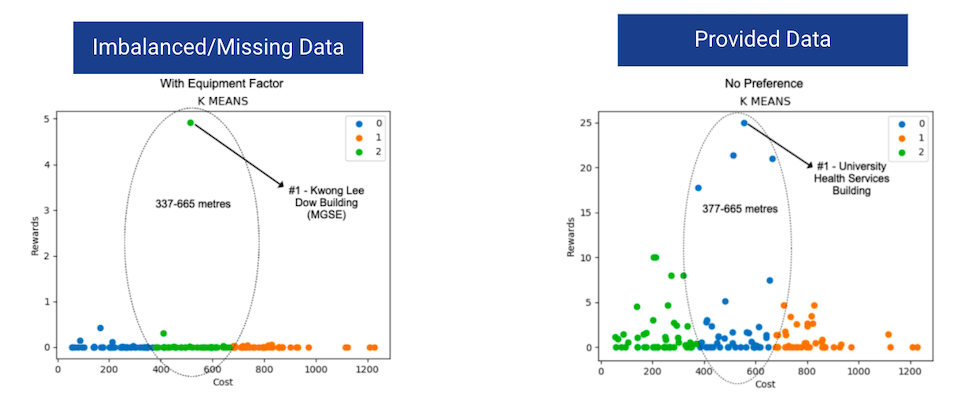
\includegraphics[width=15cm]{resources/images/algo_data.png}
\caption{Algorithm data requirements}
\label{fig:algo-data-req}
\end{figure}

\subsection{Limitations of the Algorithm}

Our algorithm relies on the assumption that the graph is a specialized weighted directed graph with one central node ($0$ in-degree and $n$ out-degree) and $n$ isolated nodes connected with only one central node. Due to this assumption, the algorithm is efficient and applicable only for such versions of the specialized graph and cannot be extended implicitly to any general weighted directed graph.
